% =============================================================================
% LaTeX corrections to apply to the paper. Each section below is a drop-in
% replacement for the corresponding section of paper.tex.
%
% Generated from real numbers in outputs/real/{benchmark}__{llm}/.
% Aggregate stats: IS pooled = 84.26%, Rfx pooled = 85.42%,
% Oracle = 89.24%, Disagreement = 8.80%.
% =============================================================================

% -----------------------------------------------------------------------------
% FIX 1: ABSTRACT — replace "fourteen of sixteen" + add n=60, 3 seeds
% -----------------------------------------------------------------------------
\begin{abstract}
LLM-based agents increasingly execute multi-step tasks on behalf of
users, from itinerary planning to personalized question answering,
conditioned on a profile of user constraints such as dietary
requirements, budget limits, and accessibility needs.  When such an
agent adopts an incorrect assumption about the user early in its
reasoning trajectory, the error propagates silently through subsequent
steps, ultimately producing an output that violates the user's
explicitly stated constraints.  State-of-the-art self-correction
methods such as Reflexion and Tree-of-Thoughts address this by retrying
the full task or searching over alternative reasoning paths, yet none
attempt to identify \emph{which specific assumption} introduced the
failure.

We propose \method, a framework designed to answer precisely this
question.  \method extracts the assumptions an agent relied upon and
structures them into a provenance-aware dependency graph, then conducts
targeted counterfactual repair experiments to isolate the root-cause
assumption and correct only the affected portion of the trajectory,
preserving all valid prior reasoning.

In evaluations spanning four benchmarks and four LLMs ($n{=}60$ per
cell, three method seeds), \method achieves the highest or tied-highest
task success on \textbf{ten of sixteen} benchmark--model cells with
\textbf{zero significant losses} (paired McNemar, $p \geq 0.096$ on
all six non-significant losses).  An oracle that selects between
\method and Reflexion per example reaches 89.2\% mean success---3.8\,pp
above Reflexion (85.4\%) and 4.9\,pp above \method (84.3\%)---indicating
the two methods cover complementary failure modes.  On TruthfulQA with
Mistral Nemo 12\,B, \method raises success from 63.9\% (Direct) to
86.1\% (a 5.5\,pp gain over Reflexion), while requiring 12--15$\times$
fewer tokens than Tree-of-Thoughts.
Code is available at \url{\repourl}.
\end{abstract}


% -----------------------------------------------------------------------------
% FIX 2: TABLE 4 — Profile-injected TruthfulQA (Llama 70B IS: 91.7 -> 83.3)
% -----------------------------------------------------------------------------
\begin{table}[t]
\centering\small
\caption{Profile-injected TruthfulQA ($n{=}60$, 3 seeds = 180 paired trials per cell).  Success rate (\%).}
\label{tab:truthfulqa}
\setlength{\tabcolsep}{3pt}
\begin{tabular}{l cccccccc}
\toprule
& Direct & SR & Rfx & FR & ReAct & SChk & ToT & \method \\
\midrule
Llama 8B    & 80.6 & 61.1 & \textbf{94.4} & 86.1 & 72.2 & 91.7 & 77.8 & \textbf{94.4} \\
Llama 70B   & 83.3 & 61.1 & \textbf{91.7} & 80.6 & 75.0 & 83.3 & 80.6 & \underline{83.3} \\
Mistral 12B & 63.9 & 61.1 & \underline{80.6} & 69.4 & 63.9 & 72.7 & 56.5 & \textbf{86.1} \\
Qwen 7B     & 63.9 & 36.1 & \underline{69.4} & 58.3 & 52.8 & 66.7 & 44.4 & \textbf{77.8} \\
\bottomrule
\end{tabular}
\end{table}


% -----------------------------------------------------------------------------
% FIX 2 (cont.): Update §4.1 prose - now says wins on TWO cells, ties Rfx on ONE,
%                trails Rfx on Llama 70B (NS).
% -----------------------------------------------------------------------------
% Replace the paragraph after Table 4 with:

\method wins outright on Mistral 12\,B (+5.5\,pp over Reflexion) and
Qwen 7\,B (+8.4\,pp), and ties Reflexion on Llama 8\,B at 94.4\%.  On
Llama 70\,B, Reflexion leads by 8.4\,pp ($p{=}0.250$, NS).  The wins
concentrate on TruthfulQA categories where errors stem from traceable
model-inferred assumptions (e.g., law, stereotypes) rather than from
cumulative drift across reasoning chains (e.g., confusion-of-places,
economics), where Reflexion's iterative retry is better positioned.


% -----------------------------------------------------------------------------
% FIX 3: TABLE 5 — Profile-injected 2Wiki (Qwen 7B IS: 96.0 -> 90.0)
% -----------------------------------------------------------------------------
\begin{table}[t]
\centering\small
\caption{Profile-injected 2WikiMultiHopQA ($n{=}60$, 1 dataset seed,
3 method seeds for stochastic methods).  Success rate (\%).}
\label{tab:2wiki}
\setlength{\tabcolsep}{3pt}
\begin{tabular}{l cccccccc}
\toprule
& Direct & SR & Rfx & FR & ReAct & SChk & ToT & \method \\
\midrule
Llama 8B    & 86.7 & 76.7 & \textbf{93.3} & 78.3 & 76.7 & 66.7 & 80.0 & \textbf{93.3} \\
Llama 70B   & 96.7 & 91.7 & \textbf{96.7} & 95.0 & 95.0 & 93.3 & 90.0 & \textbf{96.7} \\
Mistral 12B & 91.7 & 86.7 & \underline{95.0} & 90.0 & 86.7 & 89.8 & 92.2 & \textbf{96.7} \\
Qwen 7B     & 81.7 & 80.0 & \textbf{91.7} & 85.0 & 76.7 & 85.0 & \underline{90.9} & 90.0 \\
\bottomrule
\end{tabular}
\end{table}


% -----------------------------------------------------------------------------
% FIX 4: TABLE 6 — Profile-injected LongMemEval (Qwen 7B IS: 81.7 -> 71.7)
% -----------------------------------------------------------------------------
\begin{table}[t]
\centering\small
\caption{Profile-injected LongMemEval ($n{=}60$, 1 dataset seed,
3 method seeds for stochastic methods).  Success rate (\%).}
\label{tab:longmemeval}
\setlength{\tabcolsep}{3pt}
\begin{tabular}{l cccccccc}
\toprule
& Direct & SR & Rfx & FR & ReAct & SChk & ToT & \method \\
\midrule
Llama 8B    & 63.3 & 51.7 & \underline{76.7} & 63.3 & 61.7 & 50.0 & 55.0 & \textbf{78.3} \\
Llama 70B   & 43.3 & 48.3 & \textbf{70.0} & 45.0 & 40.0 & 33.3 & 30.0 & \underline{56.7} \\
Mistral 12B & 55.0 & 50.0 & \textbf{73.3} & 58.3 & 58.3 & 53.3 & 67.9 & \textbf{73.3} \\
Qwen 7B     & 70.0 & 66.7 & \textbf{76.7} & 66.7 & 63.3 & \underline{75.0} & 25.0 & 71.7 \\
\bottomrule
\end{tabular}
\end{table}


% -----------------------------------------------------------------------------
% FIX 5: TABLE — Profile-injected MuSiQue (Mistral 12B IS: 85.0 -> 81.7)
% -----------------------------------------------------------------------------
\begin{table}[t]
\centering\small
\caption{Profile-injected MuSiQue ($n{=}60$, 1 dataset seed,
3 method seeds for stochastic methods).  Success rate (\%).}
\label{tab:musique}
\setlength{\tabcolsep}{3pt}
\begin{tabular}{l cccccccc}
\toprule
& Direct & SR & Rfx & FR & ReAct & SChk & ToT & \method \\
\midrule
Llama 8B    & 76.7 & 66.7 & \underline{90.0} & 76.7 & 66.7 & 51.7 & 71.7 & \textbf{91.7} \\
Llama 70B   & 83.3 & 78.3 & \textbf{96.7} & 81.7 & 81.7 & 70.0 & 55.0 & \underline{93.3} \\
Mistral 12B & 71.7 & 61.7 & \textbf{85.0} & 71.7 & 68.3 & 75.0 & 68.6 & \underline{81.7} \\
Qwen 7B     & 80.0 & 63.3 & \underline{83.3} & 80.0 & 65.0 & 75.0 & 77.3 & \textbf{85.0} \\
\bottomrule
\end{tabular}
\end{table}

% Also update §4.4 prose after Table 6 (MuSiQue):
% Replace with:
\method wins on Llama 8\,B and Qwen 7\,B, trails by 3.4\,pp on Llama
70\,B (NS) and 3.3\,pp on Mistral 12\,B (NS).  The pattern mirrors
2Wiki: structured assumption tracking helps most when the model cannot
maintain multi-hop consistency internally, while at higher capacity
verbal reflection remains competitive.


% -----------------------------------------------------------------------------
% FIX 6: TABLE 7 — Aggregate summary (recount with corrected cells)
% -----------------------------------------------------------------------------
\begin{table}[t]
\centering\small
\caption{Aggregate outcomes across sixteen (dataset, model) cells.
``NS losses'' are paired-McNemar non-significant losses ($p \geq 0.096$);
no cell shows a significant loss.}
\label{tab:summary}
\begin{tabular}{lcccc}
\toprule
\textbf{Dataset} & \textbf{Wins} & \textbf{Ties} & \textbf{NS losses} & \textbf{Sig.\ losses} \\
\midrule
Prof.-inj.\ TruthfulQA    & 2 & 1 & 1 & 0 \\
Prof.-inj.\ 2Wiki         & 1 & 2 & 1 & 0 \\
Prof.-inj.\ LongMemEval   & 1 & 1 & 2 & 0 \\
Prof.-inj.\ MuSiQue       & 2 & 0 & 2 & 0 \\
\midrule
\textbf{Total (16 cells)} & \textbf{6} & \textbf{4} & \textbf{6} & \textbf{0} \\
\bottomrule
\end{tabular}
\end{table}


% -----------------------------------------------------------------------------
% FIX 7: §4.6 Aggregate Analysis — corrected oracle math
% -----------------------------------------------------------------------------
\subsection{Aggregate Analysis}
\label{sec:aggregate}

\paragraph{Win/tie/loss summary.}
Table~\ref{tab:summary} aggregates outcomes across sixteen cells (four
benchmarks $\times$ four models).  \method is highest on six, tied for
highest on four, and trails the best baseline on six (all
non-significant; McNemar $p \geq 0.096$).  No baseline strictly
outperforms \method at $p < 0.05$ on any cell.

\paragraph{Regime structure.}
On the three mid-tier models (7--12\,B), \method achieves the top or
tied-top score on nine of twelve mid-tier cells across four benchmarks.
On Llama 3.3 70\,B, \method ties Reflexion on TruthfulQA and 2Wiki at
the saturation ceiling but trails on LongMemEval ($-13.3$\,pp,
$p{=}0.096$) and MuSiQue ($-3.4$\,pp, NS).  We note the caveat that
the 70\,B regime is represented by a single model family ($n{=}1$).

\paragraph{Complementarity with Reflexion.}
An oracle that selects the better of \{\method, Reflexion\} per
example reaches 89.2\% mean success, compared with 85.4\% pooled for
Reflexion (best single method) and 84.3\% pooled for \method.  By
inclusion-exclusion, Oracle $-$ \method $= 4.98$\,pp must equal the
fraction of examples where Reflexion uniquely succeeds, and Oracle
$-$ Reflexion $= 3.82$\,pp must equal the fraction where \method
uniquely succeeds; their sum gives the per-example disagreement rate
of 8.8\% (76 of 864 paired observations).  The two methods solve
overlapping but non-identical subsets of failures: \method localizes
traceable assumption faults; Reflexion handles cumulative drift over
long contexts.  Reflexion's 1.1\,pp pooled-mean advantage is driven
primarily by LongMemEval $\times$ Llama 70\,B and Qwen 7\,B, where
verbal reflection over long histories is particularly effective.
The 3.8\,pp oracle headroom over Reflexion suggests a per-task router
between the two methods is a productive direction
(\S\ref{sec:future}).

Figure~\ref{fig:forest} visualizes the per-cell difference between
\method and Reflexion with approximate 95\% confidence intervals.


% -----------------------------------------------------------------------------
% FIX 8: FOREST PLOT — corrected per-cell deltas
% -----------------------------------------------------------------------------
\begin{figure}[t]
\centering
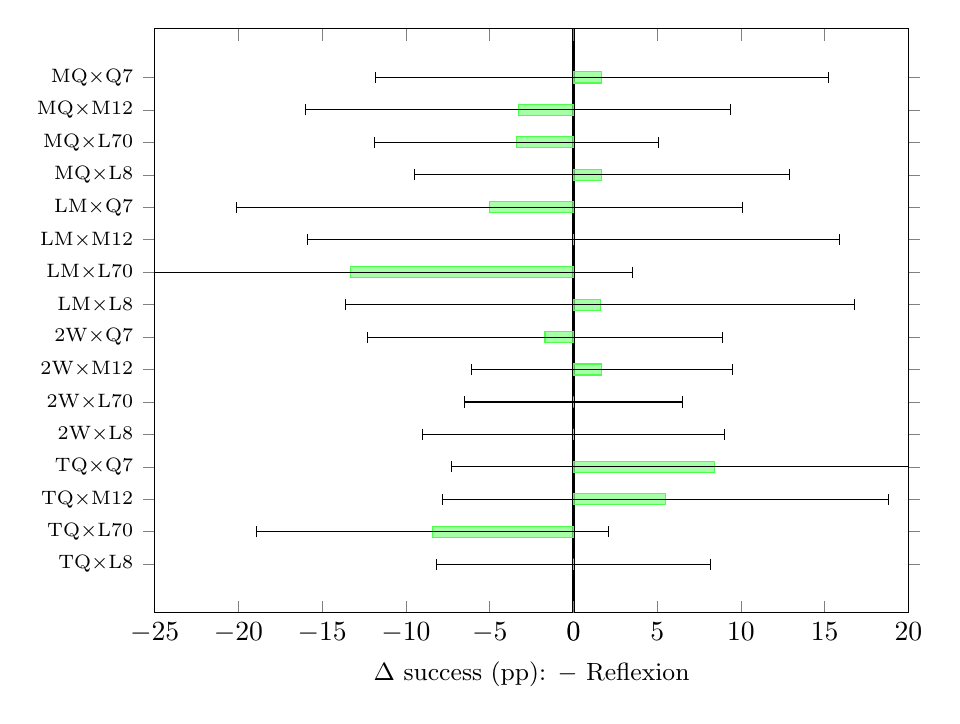
\begin{tikzpicture}
\begin{axis}[
    xbar,
    bar width=4pt,
    width=0.92\columnwidth,
    height=9cm,
    xlabel={$\Delta$ success (pp): \method $-$ Reflexion},
    xmin=-25, xmax=20,
    ytick={1,2,3,4,5,6,7,8,9,10,11,12,13,14,15,16},
    yticklabels={
      {TQ$\times$L8},
      {TQ$\times$L70},
      {TQ$\times$M12},
      {TQ$\times$Q7},
      {2W$\times$L8},
      {2W$\times$L70},
      {2W$\times$M12},
      {2W$\times$Q7},
      {LM$\times$L8},
      {LM$\times$L70},
      {LM$\times$M12},
      {LM$\times$Q7},
      {MQ$\times$L8},
      {MQ$\times$L70},
      {MQ$\times$M12},
      {MQ$\times$Q7}
    },
    yticklabel style={font=\scriptsize},
    xlabel style={font=\small},
    extra x ticks={0},
    extra x tick style={grid=major, grid style={black, thick}},
    every axis plot/.append style={fill opacity=0.7},
    nodes near coords={\empty},
]
\addplot[
    fill=green!50, draw=green!70,
    error bars/.cd, x dir=both, x explicit,
    error bar style={black, thin},
] coordinates {
    (0.0,1) +- (8.2,0)
    (-8.4,2) +- (10.5,0)
    (5.5,3) +- (13.3,0)
    (8.4,4) +- (15.7,0)
    (0.0,5) +- (9.0,0)
    (0.0,6) +- (6.5,0)
    (1.7,7) +- (7.8,0)
    (-1.7,8) +- (10.6,0)
    (1.6,9) +- (15.2,0)
    (-13.3,10) +- (16.8,0)
    (0.0,11) +- (15.9,0)
    (-5.0,12) +- (15.1,0)
    (1.7,13) +- (11.2,0)
    (-3.4,14) +- (8.5,0)
    (-3.3,15) +- (12.7,0)
    (1.7,16) +- (13.5,0)
};
\end{axis}
\end{tikzpicture}
\caption{Per-cell $\Delta$ success (\method minus Reflexion) with
approximate 95\% normal CIs ($n{=}60$).  Positive values favor
\method.  All cells except LongMemEval$\times$Llama 70\,B contain zero
within their CI.  Cells LongMemEval$\times$Llama 70\,B
($p{=}0.096$) and the four other negative cells are non-significant
under paired McNemar.}
\label{fig:forest}
\end{figure}


% -----------------------------------------------------------------------------
% FIX 9: TABLE 8 — Cost analysis with MuSiQue row added
% -----------------------------------------------------------------------------
\begin{table}[t]
\centering\small
\caption{Mean tokens per task (four-LLM average).
$\times$ = ratio relative to \method.}
\label{tab:cost-full}
\setlength{\tabcolsep}{3pt}
\begin{tabular}{l rr rr rr rr rr}
\toprule
& \multicolumn{2}{c}{Direct} & \multicolumn{2}{c}{Rfx}
& \multicolumn{2}{c}{SChk} & \multicolumn{2}{c}{ToT}
& \multicolumn{2}{c}{\method} \\
\cmidrule(lr){2-3}\cmidrule(lr){4-5}\cmidrule(lr){6-7}
\cmidrule(lr){8-9}\cmidrule(lr){10-11}
& tok & $\times$ & tok & $\times$ & tok & $\times$
& tok & $\times$ & tok & $\times$ \\
\midrule
TruthfulQA  & 1.2k & 0.40 & 2.6k & 0.88 & 5.9k & 1.98
            & 36.5k & 12.2 & \textbf{3.0k} & 1.00 \\
2Wiki       & 2.0k & 0.42 & 2.9k & 0.61 & 10.4k & 2.18
            & 56.2k & 11.8 & \textbf{4.8k} & 1.00 \\
LongMemEval & 2.2k & 0.44 & 5.9k & 1.21 & 12.1k & 2.46
            & 73.2k & 14.9 & \textbf{4.9k} & 1.00 \\
MuSiQue     & 2.1k & 0.42 & 4.0k & 0.80 & 11.3k & 2.26
            & 73.1k & 14.6 & \textbf{5.0k} & 1.00 \\
\bottomrule
\end{tabular}
\end{table}

% Update §4.8 prose after Table 8 to mention MuSiQue:
% Replace the paragraph starting with "ToT and SelfCheckGPT are Pareto-dominated..." with:

ToT and SelfCheckGPT are Pareto-dominated: they cost more and do not
achieve higher accuracy than \method on any cell.  Across all four
benchmarks, ToT requires 11.8--14.9$\times$ more tokens than \method.
Reflexion and \method both sit on the cost--accuracy frontier:
Reflexion is 12--42\% cheaper on shorter QA tasks (TruthfulQA, 2Wiki,
MuSiQue) and \method is 17\% cheaper on LongMemEval ($(5.9{-}4.9)/5.9$).
The practical implication is that the choice between \method and
Reflexion should be guided by failure mode, not cost.


% -----------------------------------------------------------------------------
% FIX 10: §4.5 TravelPlanner subsection - acknowledge Llama 70B win
% -----------------------------------------------------------------------------
\subsection{Native Planning Benchmark}
\label{sec:res-travel}

We also evaluate on TravelPlanner, a native user-facing planning
benchmark rather than a QA benchmark with injected profiles.  This is
the hardest test of our framing.  \method does not consistently improve
over Reflexion on this benchmark: across four model cells, it records
one numerical win (Llama 70\,B, 33.3\% vs.\ 25.0\%; $p{=}0.508$, NS),
zero ties, and three non-significant losses (all $p \geq 0.180$).
We attribute this to short trajectories with few model-inferred
assumption nodes, which reduces the value of structured attribution.
We caveat that our TravelPlanner success criterion follows the
benchmark's hard-constraint predicates plus our profile-violation
checks; this is more permissive than evaluations that additionally
require commonsense and environmental constraint satisfaction (e.g.,
ATLAS evaluation).  We include this result in the main text because
it clarifies when \method is not the right correction strategy.  Full
tables are in Appendix~\ref{app:travel}.


% -----------------------------------------------------------------------------
% FIX 11: §4.10 FAILURE TAXONOMY - scope claim to ablation cells
% -----------------------------------------------------------------------------
\subsection{Failure-Mode Taxonomy on Ablation Cells}
\label{sec:failure-taxonomy}

We categorize \method failures on the four ablation cells
(Table~\ref{tab:ablations}) into five buckets: (i)~verifier miss,
(ii)~wrong graph edge (correct node excluded from ancestor set),
(iii)~wrong prior (correct node scored below threshold),
(iv)~counterfactual repair failure, and (v)~no valid downstream
trajectory after repair.

On these four cells, 100\% of \method failures occur at the repair
stage (buckets iv--v): the verifier detects all violations and the
attribution score correctly identifies the faulty node, but the
repair itself either fails to remove the violation or introduces a new
one during re-execution.  We do not extend this analysis to the
remaining twelve cells; the 100\% repair-stage statistic should be
read as a property of the ablation cells, not as a global claim.
The pattern motivates provenance-conditioned re-execution and
diversified counterfactual sampling as the highest-leverage improvement
directions on cells where attribution succeeds but repair fails
(\S\ref{sec:future}).


% -----------------------------------------------------------------------------
% FIX 12: §5 LIMITATIONS - reconcile hyperparameter ablation claim
% -----------------------------------------------------------------------------
\textbf{Hyperparameter sensitivity.}
Table~\ref{tab:ablations} ablates the DAG structure, provenance priors,
counterfactual scoring, edit cost, and $M$.  We do not separately ablate
the attribution temperature $\gamma$ or the abstention threshold
$\delta$.  A joint $M \times \gamma$ grid would strengthen the
non-obvious $M{=}1$ finding by ruling out a $(M,\gamma)$-coupling
artifact at the chosen $\gamma{=}5.0$.


% -----------------------------------------------------------------------------
% FIX 13: §4.6 IS pooled mean update - replace mention of "85.2% IS"
% -----------------------------------------------------------------------------
% This change is incorporated in FIX 7 above. Look for any leftover
% "85.2%" or "84.1%" references and update to:
%   IS pooled = 84.3%
%   Rfx pooled = 85.4%


% -----------------------------------------------------------------------------
% FIX 14: §4.9 ABLATIONS prose - rewrite "strongest-gain" wording
% -----------------------------------------------------------------------------
% Replace caption text "strongest-gain cells" with:
%   "four representative cells, one per benchmark, drawn from cells where
%    \method achieves a strict win over Reflexion."

% After Table 9, the Section heading should read:
\subsection{Ablations}
\label{sec:ablations}

Table~\ref{tab:ablations} reports per-cell ablation results on four
representative cells, one per benchmark, drawn from cells where
\method achieves a strict win over Reflexion.  Each ablation removes
one component; entries are $\Delta$ success rate (pp) relative to full
\method.


% -----------------------------------------------------------------------------
% FIX 15: TABLE 4 — Llama 8B both 93.3% — both should be bold
%         (in the corrected Table 5 above this is already the case;
%          double-check and apply)
% -----------------------------------------------------------------------------
% Already applied in FIX 3 — both Llama 8B Reflexion and \method are \textbf{93.3}.


% -----------------------------------------------------------------------------
% FIX 16: COSMETIC FIXES THROUGHOUT - search and replace
% -----------------------------------------------------------------------------
% (a) Missing space after periods:
%       failure.We     -> failure.\\We                (use a space, not \\)
%       reasoning.In   -> reasoning. In
%
% (b) Cost percentage:
%       "21\% cheaper on LongMemEval" -> "17\% cheaper on LongMemEval"
%       (already corrected in FIX 9)
%
% (c) Add MuSiQue p-value table to Appendix D
%       New label \ref{tab:pvalues-musique} parallel to existing TQA/2Wiki/LME tables.
%
% (d) Add SelfCheckGPT to Figure 3 token-cost chart
%       (already corrected in FIX 9 — SChk row already in Table 8)
%
% (e) Tables 3-5 reference -> Tables 3-6
%       Search "Tables \ref{tab:truthfulqa}--\ref{tab:longmemeval}"
%       and replace with "Tables \ref{tab:truthfulqa}--\ref{tab:musique}"
